\section{Workload Characterization}
\label{sec:workloadchar}



Comparing the trends observed in Spider I vs Spider II



\subsection{I/O Usage Trends}



\subsubsection{Atlas1 and Atlas2 Utilization}


-- Bandwidth
-- Controller usage trends

\subsubsection{Read vs Write}

Figure~\ref{fig:rwratio} shows the read and write ratios on Spider 1 and 2
storage systems. As can be seen, on Spider 1 60\% of the I/O workload was write
operations and 40\% was reads. Spider 1 was a center-wide shared resource
across all OLCF platforms, and high percent of the read requests was attributed
to analysis and data transfer I/O workloads accessing Spider 1. 

Spider 2 is also a center-wide shared resource, and a similar trend can be
observed. However, the percent of reads on Spider 2 is less compared to Spider
1, and they amount to roughly 25\%. This can be attributed to large-data
transfers into Spider 2 from various resources currently going on for later
processing on Titan. Also it is quite visible in Figure~\ref{fig:rwratio}(b)
that Atlas1 portion of the Spider 2 is 10\% more write-intensive than the
Atlas2 (left half vs. right half of the Figure~\ref{fig:rwratio}(b). This
discrepancy is due to a user project allocation problem we encountered early
on. User projects were categorized in terms of science domains and expected I/O
requirements equally on Atlas1 and Atlas2 portions when Spider 2 was turned
into production. However, our expectation did not materialize completely, and
since then we have been observing more I/O on Atlas1 compared to Atlas2. We
have taken steps (e.g. moving some user projects from Atlas1 to Atlas2) to
rectify this mismatch and over the time it is expected that both portions will
be exercised with roughly equivalent I/O workloads. 

\begin{figure}[!t]
\begin{center}
\begin{tabular}{c}
{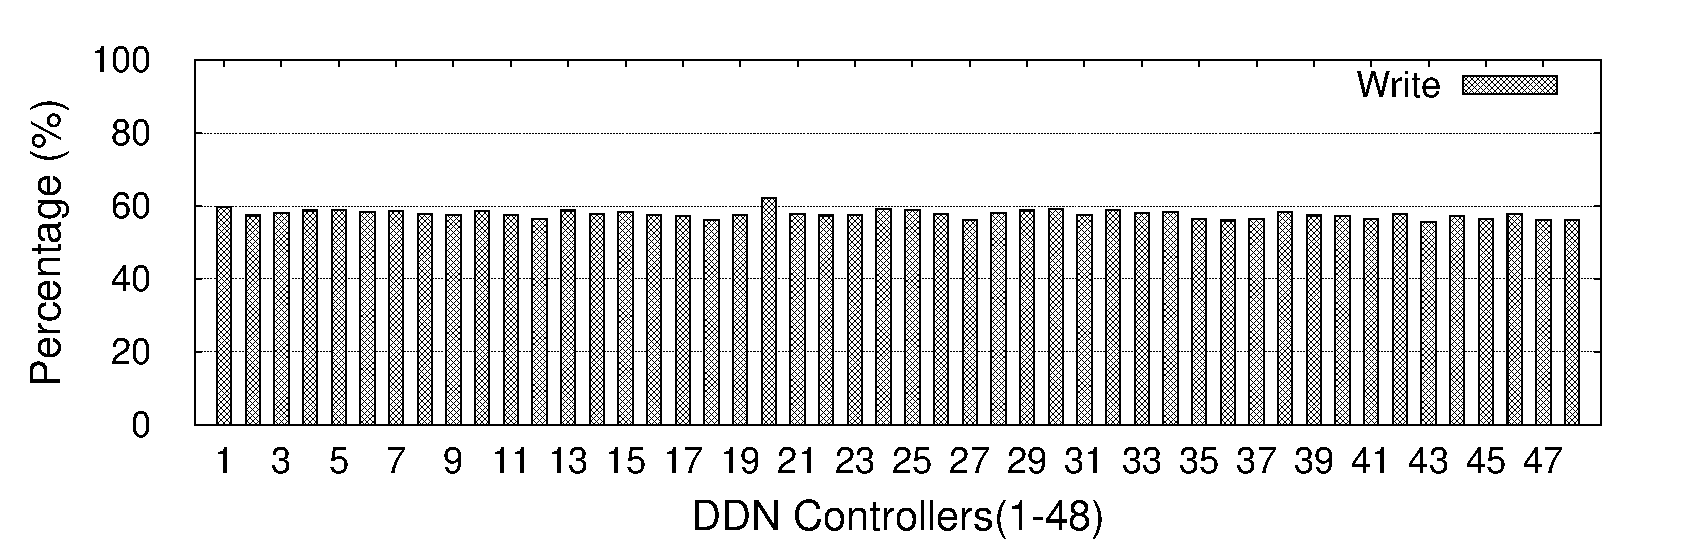
\includegraphics[width=0.5\textwidth]{./figs/spider1-wr-ratio.eps}}\\
{(a) Spider 1}\\
{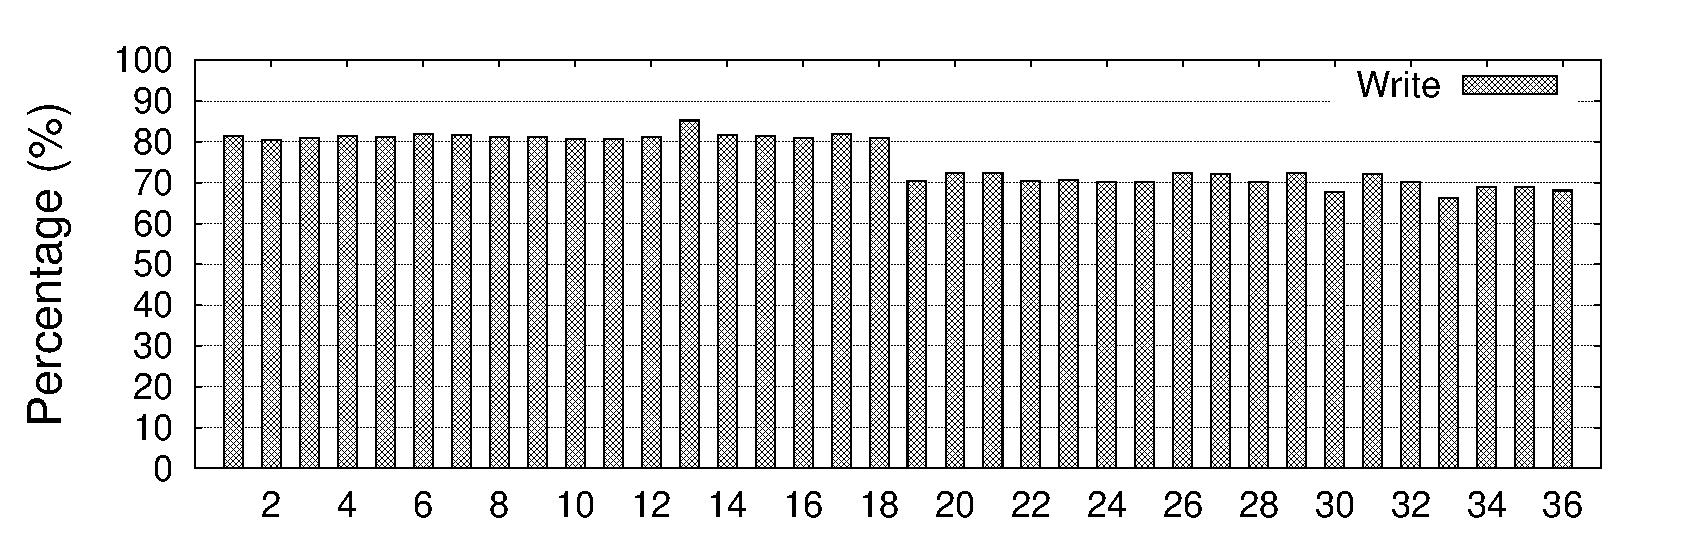
\includegraphics[width=0.5\textwidth]{./figs/spider2-wr-ratio.eps}}\\
{(b) Spider 2}\\
\end{tabular}
\vspace{-0.1in}
\caption{Read vs Write on the Storage System}
\label{fig:rwratio}
\end{center}
\end{figure}


\subsection{I/O Requests}
\subsubsection{Request Size distribution}



\begin{figure}[!t]
\begin{center}
\begin{tabular}{cc}
\hspace*{-1cm}                                                           
{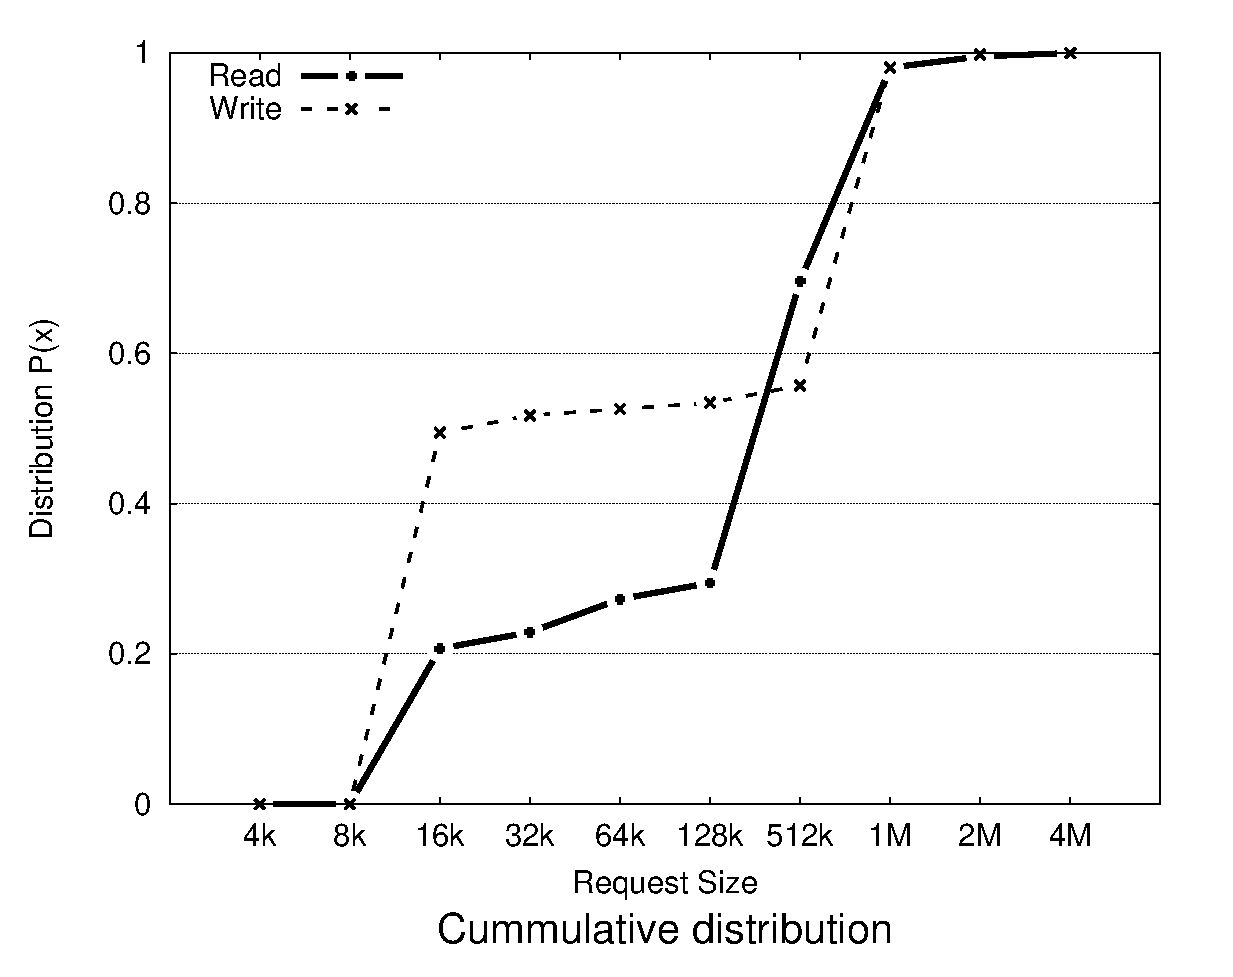
\includegraphics[width=0.27\textwidth]{./figs/spider1-reqSizeCDF.eps}}&
\hspace{-2mm}
{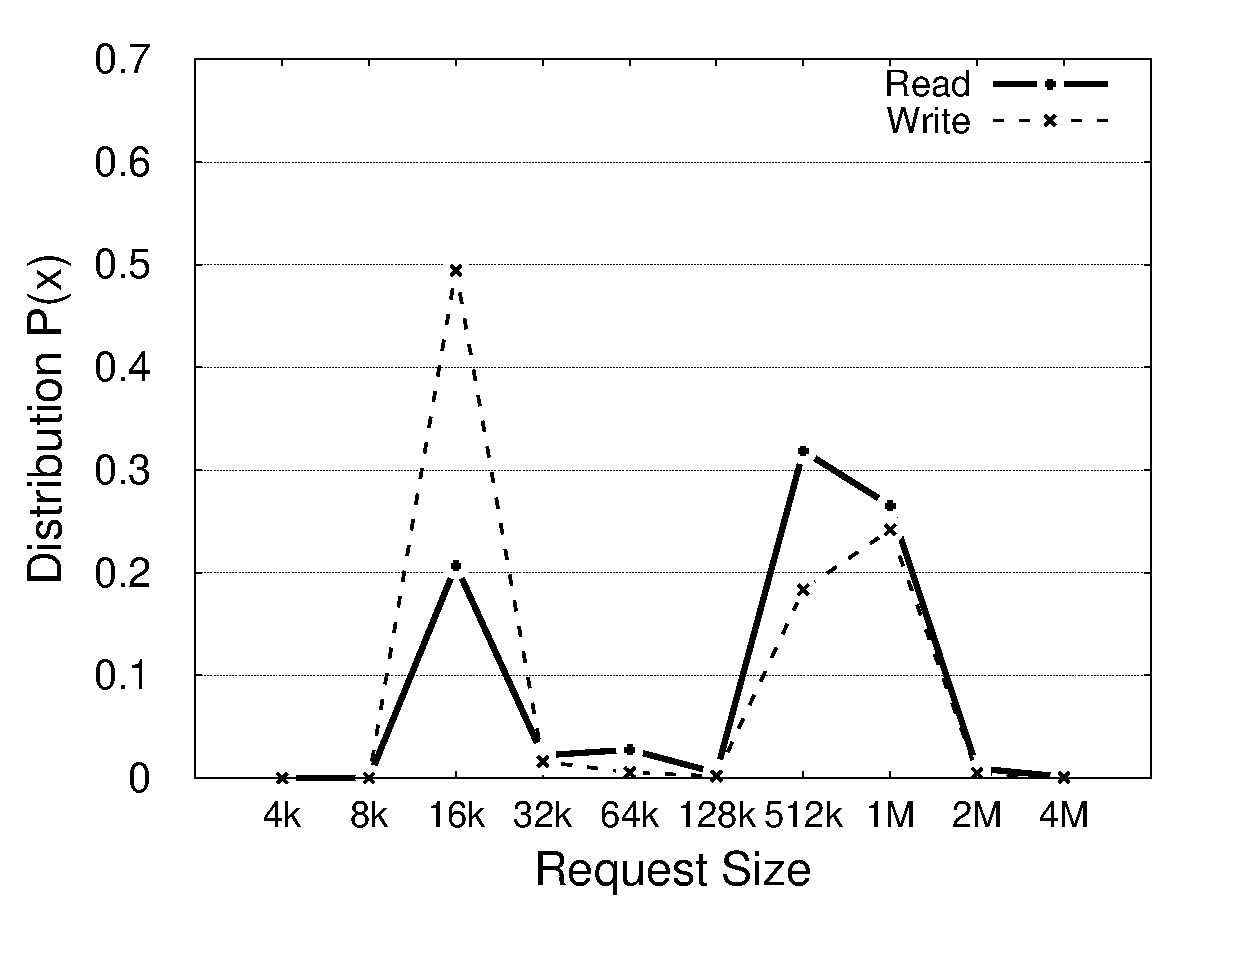
\includegraphics[width=0.27\textwidth]{./figs/spider1-reqSizePDF.eps}}\\
\small (a) CDF & \small(b) PDF \\
\end{tabular}
\vspace{-0.1in}
\captionsetup{justification=centering}
\caption{Spider 1 - Distribution of Request Sizes}
\label{fig:spider1-reqsizedist}
\end{center}
\end{figure}

\begin{figure}[!t]
\begin{center}
\begin{tabular}{cc}
\hspace*{-1cm}                                                           
{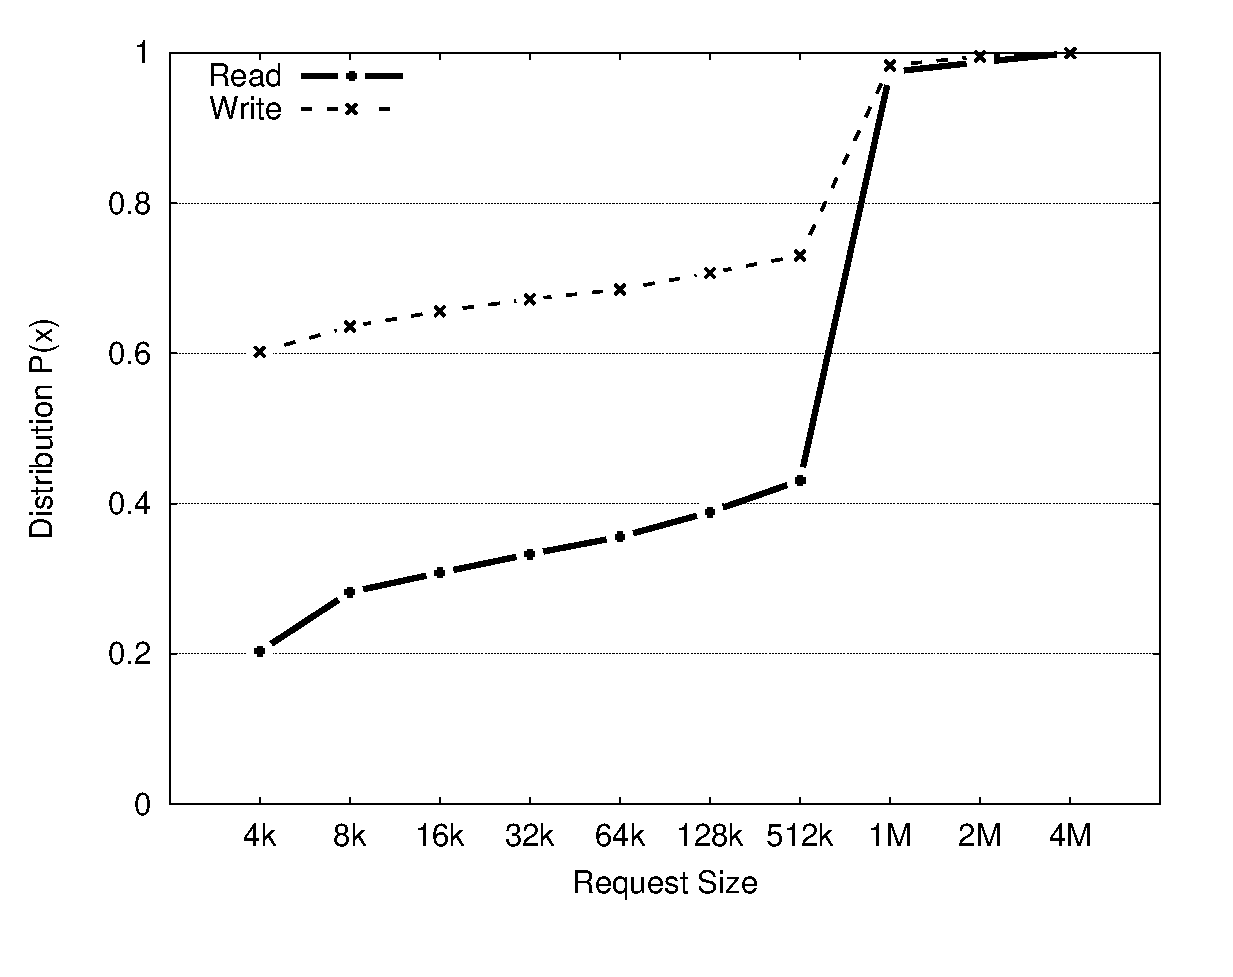
\includegraphics[width=0.27\textwidth]{./figs/spider2-reqSizeCDF.eps}}&
\hspace{-2mm}
{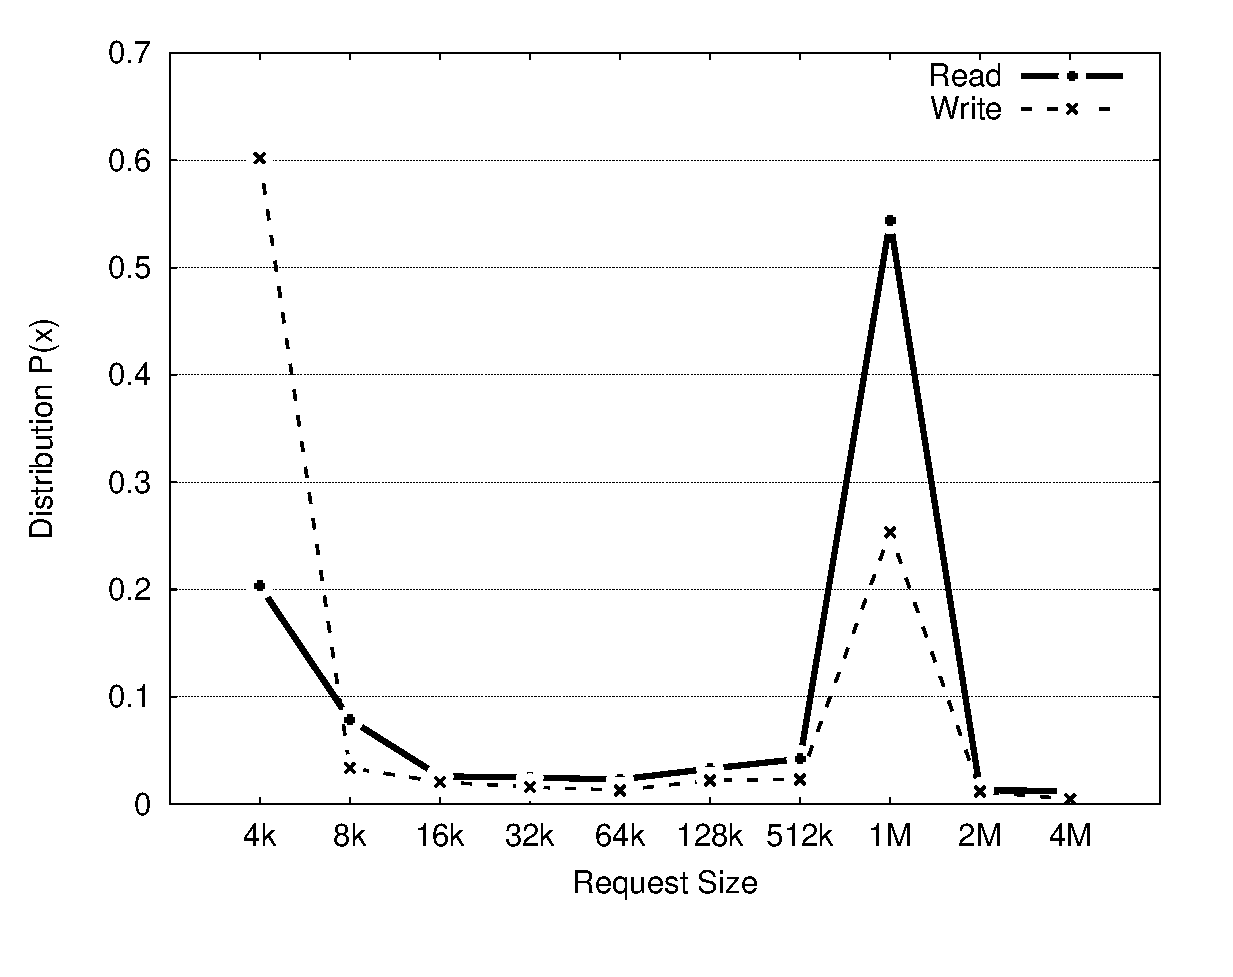
\includegraphics[width=0.27\textwidth]{./figs/spider2-reqSizePDF.eps}}\\
\small (a) CDF & \small(b) PDF \\
\end{tabular}
\vspace{-0.1in}
\caption{Spider 2 - Distribution of Request Sizes}
\label{fig:spider2-reqsizedist}
\end{center}
\end{figure}

Figure~\ref{fig:spider1-reqsizedist} and Figure~\ref{fig:spider2-reqsizedist}
shows the distribution of read and writes requests on Spider 1 and Spider 2,
respectively. As can be seen, there are differences. The Lustre file system
supports a range of request block sizes, the smallest being 4 kiloBytes (kB)
and the largest being 4 MegaBytes (MB).  However, on Spider 1, the smallest
block size we were able to monitor was 16KB, a limitation of the DDN RAID
controller. Interpreting from the CDF and PDF plots here are some interesting
observation.

\begin{itemize}

\item  60\% of write requests on Spider 2 are 4kB or less.  In Spider 1, we
unable to distinguish between the 4kB, 8kB and 16kB, which accounted for 50\%
of the write requests. Accounting for this and comparing Spider 1 and 2 file
size distributions, it can be seen that there is 10\% more small files (i.e.
smaller than 8kB) on Spider 2, for write operations. Please remember that these
are directly obtained from the DDN controllers not from the file system. One
possible explanation for this increase can be due to the local file system
(ldiskfs) metadata operations. Other possible explanation can be the
controller-level background disk integrity check (i.e. scrubbing) events. Exact
cause of this increase is unknown at this point and it is being investigated.
For read operations, Spider 1 and Spider 2 behave the same for small files, the
distribution has not changed.

\item  For writes, Spider 2 has 70\% of the requests which are less than or
equal to 512kB, whereas on Spider 1, only 55\% of the requests were less than
512kB. <Have no explanation for this. Maybe Jason/Dustin has something?> 

\item   On Spider 1, we observed a large number of 512kB requests for both read
and write requests. This was due to the SRP we were running on Spider 1. SRP at
the time was not able to queue 1024 requests and maximum allowed was 512. This
problem has been fixed since then in the kernel and on Spider 2 the number of
512kB requests has been dramatically reduced, as a result.

\item On Spider 2 over 50\% of reads were 1MB, similar to Spider 1 combined
512kB and 1MB were 50\%. However, only 25\% of writes on Spider 2 are 1MB,
whereas on Spider 1 over 45\% of writes where either 512kB or 1MB. <Have no explanation for this. Maybe Jason/Dustin has something?>

\end{itemize}


\subsubsection{Request Size Latency distribution}

\begin{figure}[!t]
\centering
\begin{tabular}{cc}
{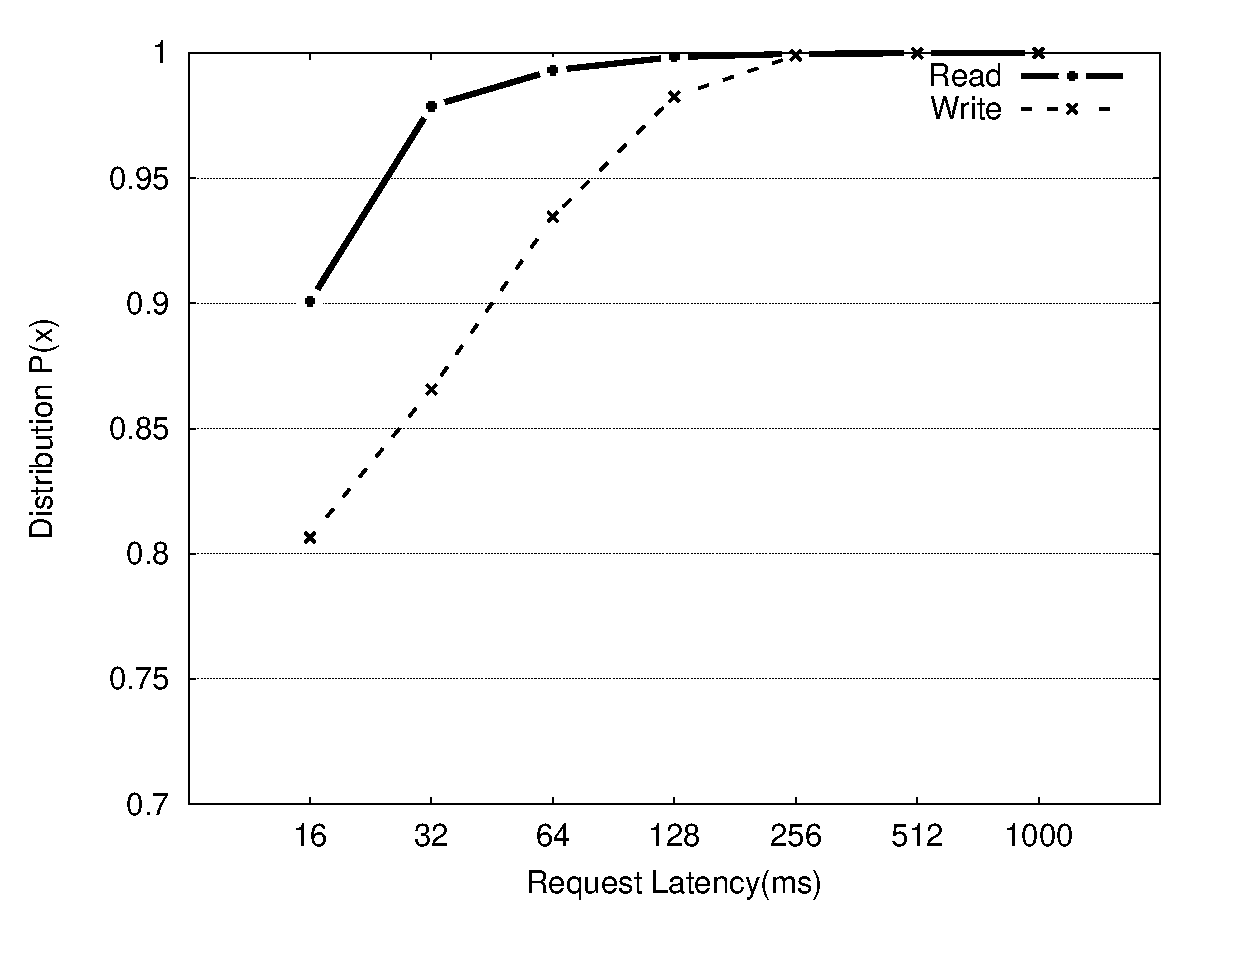
\includegraphics[width=0.24\textwidth]{./figs/spider2-reqLatCDF.eps}}&
{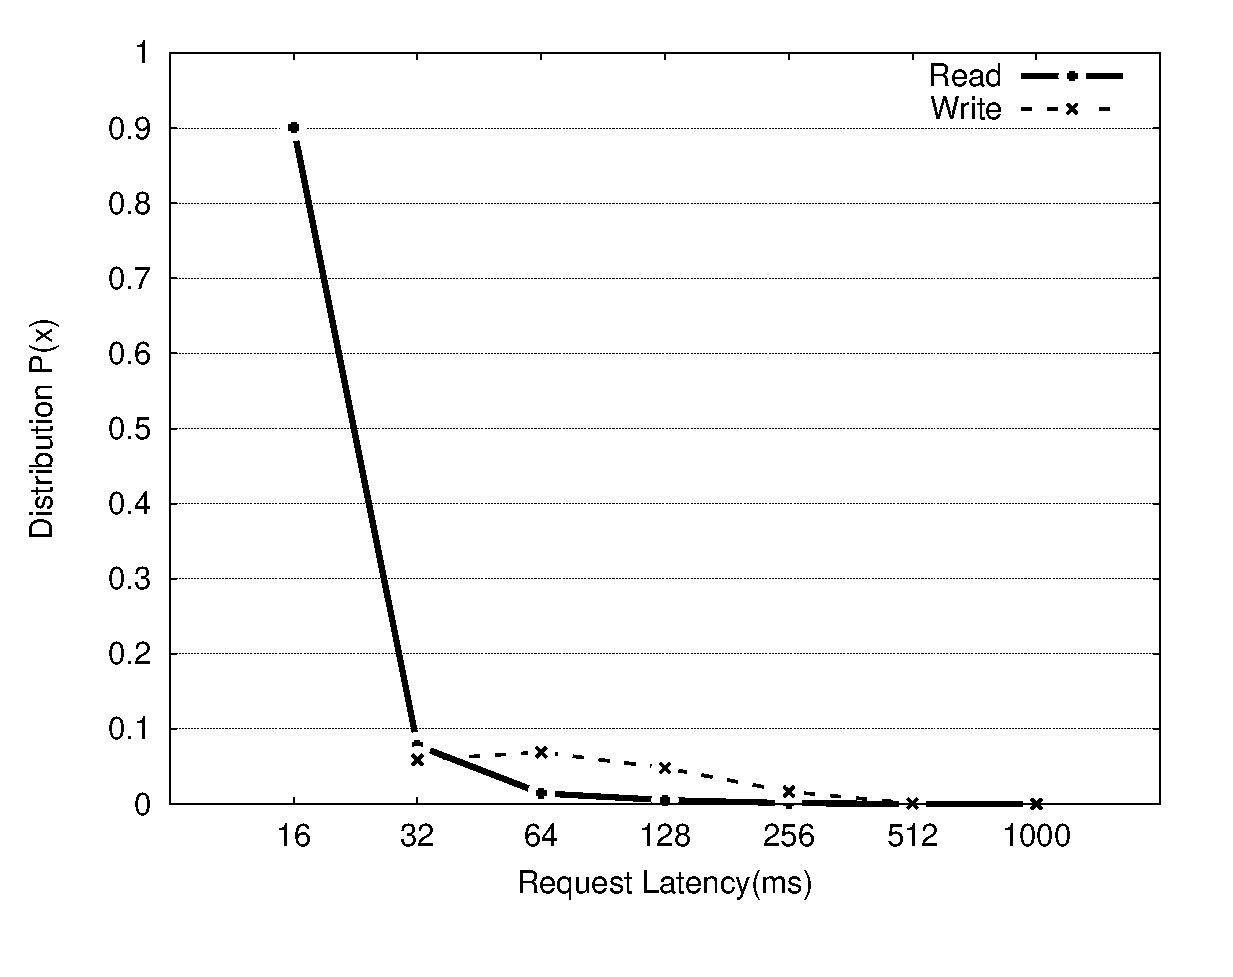
\includegraphics[width=0.24\textwidth]{./figs/spider2-reqLatPDF.eps}}\\
\end{tabular}
\vspace{-0.1in}
\centering
\caption{Spider 2 - Request Service Latency distribution}
\label{fig:spider1-reqLat}
\end{figure}




\subsection{Request Size vs Bandwidth}

 
